% Sostituisco i placeholder registrati con la specifica variabile per il documento corrente. Questa parte iniziale contiene intestazioni e templates.

% Modificare ad ogni modifica e documento
\newcommand{\documento}{\PdP}
\newcommand{\nomedocumentofisico}{PianoDiProgetto 0\_0\_5.pdf}
\newcommand{\redazione}{\DS \\ & \MC \\ & \DAN}
\newcommand{\verifica}{\AS \\ & \NS}
\newcommand{\versione}{0.0.5}
\newcommand{\approvazione}{\AS}
\newcommand{\uso}{Esterno}
\newcommand{\destinateTo}{\TV, \\ & \RC, \\ & \IS}
\newcommand{\datacreazione}{02 Dicembre 2016}
\newcommand{\datamodifica}{21 Dicembre 2016}
\newcommand{\stato}{Non approvato}

%Abilitazione indice delle tabelle e figure
\def\TABELLE{false}
\def\FIGURE{false}

%Inclusione di layout e variabili (Non modificare)
%Stile e dimensione del documento
\documentclass[a4paper,11pt]{article}

%Pacchetti da importare
\usepackage{ifthen}
\usepackage[italian]{babel}
\usepackage[utf8]{inputenc}
\usepackage[T1]{fontenc}
\usepackage{float}
\usepackage{chapterbib}
\usepackage{graphicx}
\usepackage[a4paper,top=2.5cm,bottom=2.5cm,left=2.5cm,right=2.5cm]{geometry}
\usepackage[colorlinks=true, urlcolor=black, citecolor=black, linkcolor=black]{hyperref}
\usepackage{booktabs}
\usepackage{fancyhdr}
\usepackage{totpages}
\usepackage{tabularx, array}
\usepackage{dcolumn}
\usepackage{epstopdf}
\usepackage{booktabs}
\usepackage{fancyhdr}
\usepackage{longtable}
\usepackage{calc}
\usepackage{datatool}
\usepackage[bottom]{footmisc}
\usepackage{listings}
\usepackage{textcomp}
\usepackage{titlesec}
\usepackage{rotating}
\usepackage{multirow}
\usepackage{placeins}
\usepackage{color}
\usepackage[table,usenames,dvipsnames]{xcolor}
\usepackage{hyperref}
\usepackage{makecell}
\usepackage{breakurl}
\usepackage{hyperref}
\usepackage{multirow}
\usepackage{xcolor,colortbl}
\usepackage{afterpage}



%Stile fancy per il documento (Header e footer)
\pagestyle{fancy}
%Rimuovo l'indentazione
\setlength{\parindent}{0pt}

%Imposto l'intestazione
\lhead{\Large{\progetto} \\ \footnotesize{\documento}}
%Linea sotto l'intestazione
\renewcommand{\headrulewidth}{0.4pt} 

%Footer
\lfoot{\textit{\gruppoLink}\\ \footnotesize{\email}}
%Footer con numero romano per le prime pagine
\rfoot{\thepage}
\cfoot{}
%Linea sopra il footer
\renewcommand{\footrulewidth}{0.4pt}   

%Imposta il livello degli elenchi 
\setcounter{secnumdepth}{7}
\setcounter{tocdepth}{7}

%Paragrafi impostati come una sezione
\titleformat{\paragraph}{\normalfont\normalsize\bfseries}{\theparagraph}{1em}{}
\titlespacing*{\paragraph}{0pt}{3.25ex plus 1ex minus .2ex}{1.5ex plus .2ex}

\titleformat{\subparagraph}{\normalfont\normalsize\bfseries}{\thesubparagraph}{1em}{}
\titlespacing*{\subparagraph}{0pt}{3.25ex plus 1ex minus .2ex}{1.5ex plus .2ex}

\makeatletter
\newcounter{subsubparagraph}[subparagraph]
\renewcommand\thesubsubparagraph{
  \thesubparagraph.\@arabic\c@subsubparagraph}
\newcommand\subsubparagraph{
  \@startsection{subsubparagraph}
    {6}
    {\parindent}
    {3.25ex \@plus 1ex \@minus .2ex}
    {0.75em}
    {\normalfont\normalsize\bfseries}}
\newcommand\l@subsubparagraph{\@dottedtocline{6}{10em}{5.5em}} 
\newcommand{\subsubparagraphmark}[1]{}
\makeatother

\makeatletter
\newcounter{subsubsubparagraph}[subsubparagraph]
\renewcommand\thesubsubsubparagraph{
  \thesubsubparagraph.\@arabic\c@subsubsubparagraph}
\newcommand\subsubsubparagraph{
  \@startsection{subsubsubparagraph}
    {7}
    {\parindent}
    {3.25ex \@plus 1ex \@minus .2ex}
    {0.75em}
    {\normalfont\normalsize\bfseries}}
\newcommand\l@subsubsubparagraph{\@dottedtocline{7}{10em}{6.5em}}
\newcommand{\subsubsubparagraphmark}[1]{}
\makeatother

%Variabili generali
\newcommand{\progetto}{API Market}
\newcommand{\gruppo}{NetBreak}
\newcommand{\gruppoLink}{\href{https://git.io/v1Rgz}{NetBreak}}
\newcommand{\email}{netbreakswe@gmail.com}

%Variabili riguardanti i documenti
\newcommand{\AdR}{Analisi dei Requisiti}
\newcommand{\NdP}{Norme di Progetto}
\newcommand{\PdP}{Piano di Progetto}
\newcommand{\SdF}{Studio di Fattibilità}
\newcommand{\PdQ}{Piano di Qualifica}
\newcommand{\VI}{Verbale Interno}
\newcommand{\VE}{Verbale Esterno}
\newcommand{\ST}{Specifica Tecnica}
\newcommand{\DDP}{Definizione di Prodotto}
\newcommand{\MU}{Manuale Utente}
\newcommand{\G}{Glossario}
\newcommand{\LdP}{Lettera di Presentazione}

%Variabili per i membri del gruppo
\newcommand{\AS}{Andrea Scalabrin}
\newcommand{\NS}{Nicolò Scapin}
\newcommand{\AN}{Alberto Nicolè}
\newcommand{\DS}{Davide Scarparo}
\newcommand{\DAN}{Dan Serbanoiu}
\newcommand{\MC}{Marco Casagrande}

%Ruoli di progetto
\newcommand{\RdP}{Responsabile di Progetto}
\newcommand{\Res}{Responsabile}
\newcommand{\Amm}{Amministratore}
\newcommand{\Ver}{Verificatore}
\newcommand{\Prog}{Progettista}
\newcommand{\Progr}{Programmatore}
\newcommand{\Ana}{Analista}
\newcommand{\RdPs}{Responsabili di Progetto}
\newcommand{\Ress}{Responsabile}
\newcommand{\Amms}{Amministratori}
\newcommand{\Vers}{Verificatori}
\newcommand{\Progs}{Progettisti}
\newcommand{\Progrs}{Programmatori}
\newcommand{\Anas}{Analisti}

%Professori e proponente
\newcommand{\TV}{Prof. Tullio Vardanega}
\newcommand{\RC}{Prof. Riccardo Cardin}
\newcommand{\IS}{ItalianaSoftware S.r.l.}
\newcommand{\proponente}{ItalianaSoftware S.r.l.}

\newcommand{\diaryEntry}[5]{#2 & \emph{#4} & #3 & #5 & #1\\ \hline}

%Comando per una nuova riga nella tabella del changelog
\newcommand{\specialcell}[2][c]{%
	\begin{tabular}[#1]{@{}c@{}}#2\end{tabular}}

\renewcommand*\sectionmark[1]{\markboth{#1}{}}
\renewcommand*\subsectionmark[1]{\markright{#1}}

%Variabili per la fase di lavoro
\newcommand{\AR}{Analisi dei Requisiti}
\newcommand{\PA}{Progettazione Architetturale}
\newcommand{\PD}{Progettazione Architetturale Dettagliata}
\newcommand{\CO}{Codifica}
\newcommand{\VV}{Verifica e Validazione}

%Variabili per le varie revisioni
\newcommand{\RR}{Revisione dei Requisiti}
\newcommand{\RP}{Revisione di Progettazione}
\newcommand{\RPMin}{Revisione di Progettazione Minima}
\newcommand{\RPMax}{Revisione di Progettazione Massima}
\newcommand{\RQ}{Revisione di Qualifica}
\newcommand{\RA}{Revisione di Accettazione}

\newcommand{\myincludegraphics}[2][]{%
	\setbox0=\hbox{\phantom{X}}%
	\vtop{
		\hbox{\phantom{X}}
		\vskip-\ht0
		\hbox{\includegraphics[#1]{#2}}}}

\renewcommand\footnoterule{\rule{\linewidth}{1pt}}

\newcommand{\nogloxy}[1]{#1} % comando da usare per evitare di metttere il mark del glossario
\newcommand{\gloxy}[1]{\emph{#1}$_G$}

\colorlet{punct}{red!60!black}
\definecolor{background}{HTML}{EEEEEE}
\definecolor{delim}{RGB}{20,105,176}
\colorlet{numb}{magenta!60!black}
\lstdefinelanguage{json}{
	basicstyle=\small\ttfamily,
	numbers=left,
	numberstyle=\scriptsize,
	stepnumber=1,
	numbersep=8pt,
	showstringspaces=false,
	breaklines=true,
	frame=lines,
	backgroundcolor=\color{background},
	literate=
	*{0}{{{\color{numb}0}}}{1}
	{1}{{{\color{numb}1}}}{1}
	{2}{{{\color{numb}2}}}{1}
	{3}{{{\color{numb}3}}}{1}
	{4}{{{\color{numb}4}}}{1}
	{5}{{{\color{numb}5}}}{1}
	{6}{{{\color{numb}6}}}{1}
	{7}{{{\color{numb}7}}}{1}
	{8}{{{\color{numb}8}}}{1}
	{9}{{{\color{numb}9}}}{1}
	{:}{{{\color{punct}{:}}}}{1}
	{,}{{{\color{punct}{,}}}}{1}
	{\{}{{{\color{delim}{\{}}}}{1}
	{\}}{{{\color{delim}{\}}}}}{1}
	{[}{{{\color{delim}{[}}}}{1}
	{]}{{{\color{delim}{]}}}}{1},
}
\lstset{language=json}
\lstset{literate=%
	{Ö}{{\"O}}1
	{Ä}{{\"A}}1
	{Ü}{{\"U}}1
	{é}{{\"s}}1
	{è}{{\"e}}1
	{à}{{\"a}}1
	{ö}{{\"o}}1
}

\newcommand{\impl}{\textcolor{Green}{Implementato}}
\newcommand{\implno}{\textcolor{Red}{Non Implementato}}
\newcommand\Tstrut{\rule{0pt}{3.2ex}}         % = `top' strut
\newcommand\Bstrut{\rule[-1.9ex]{0pt}{0pt}}   % = `bottom' strut
\definecolor{Gray}{gray}{0.85}
\usepackage[inline]{enumitem}

%Inclusione del changelog per il documento corrente
\newcommand{\modifiche}
{	
	Approvazione documento & \specialcell[t]{\DS\\\Res} & \specialcell[t]{2017-03-04\\2.0.0}
	\\
	\hline
	Verifica documento & \specialcell[t]{\MC\\\Ver} & \specialcell[t]{2017-03-03\\1.1.0}
	\\
	\hline
	Stesura sezione "Resoconto attività di verifica" & \specialcell[t]{\DS\\\Ana} & \specialcell[t]{2017-03-01\\1.0.4}
	\\
	\hline
	Nuova stesura sezione "Qualità di prodotto" & \specialcell[t]{\NS\\\Ana} & \specialcell[t]{2017-02-28\\1.0.3}
	\\
	\hline
	Nuova stesura sezione "Qualità di processo" & \specialcell[t]{\DS\\\Ana} & \specialcell[t]{2017-02-24\\1.0.2}
	\\
	\hline
	Ristrutturazione documento secondo suggerimenti del committente & \specialcell[t]{\DS\\\Ana} & \specialcell[t]{2017-02-23\\1.0.1}
	\\
	\hline
	Approvazione documento & \specialcell[t]{\NS\\\Res} & \specialcell[t]{2017-01-03\\1.0.0}
	\\
	\hline
	Effettuate modifiche secondo verifica & \specialcell[t]{\DS\\\Ana} & \specialcell[t]{2016-12-31\\0.1.1}
	\\
	\hline
	Verifica documento & \specialcell[t]{\MC\\\Ver} & \specialcell[t]{2016-12-29\\0.1.0}
	\\
	\hline
	Creata sezione "Qualità di prodotto" & \specialcell[t]{\DS\\\Ana} & \specialcell[t]{2016-12-28\\0.0.5}
	\\
	\hline
	Creata sezione "Qualità di processo" & \specialcell[t]{\DAN\\\Ana} & \specialcell[t]{2016-12-26\\0.0.4}
	\\
	\hline
	Creata sezione "Definizione obiettivi di qualità" & \specialcell[t]{\AN\\\Ana} & \specialcell[t]{2016-12-23\\0.0.3}
	\\
	\hline
	Creata introduzione & \specialcell[t]{\AN\\\Ana} & \specialcell[t]{2016-12-22\\0.0.2}
	\\
	\hline	
	Creato template documento & \specialcell[t]{\AS\\\Res} & \specialcell[t]{2016-12-20\\0.0.1}
	\\	
	
}

%Imposto la profondità degli indici
\setcounter{secnumdepth}{7}
\setcounter{tocdepth}{7}

\begin{document}

%Inclusione del template per la homepage (Non modificare)
%Importante: Non modificare questo template
%Modificare il documento principale per cambiare le parti

\begin{center}


%Spaziatura verticale

\vspace{4em}

%Intestazione con nome del gruppo
\begin{center} 
	\begin{Huge}
		\textbf{\fontsize{15mm}{20mm}\selectfont \gruppoLink} 
	\end{Huge}
\end{center}

\begin{center}
	\begin{Large}
		\vspace{0.3em}
		\textbf{Progetto \progetto}
	\end{Large}
\end{center}

%Inclusione del logo

\includegraphics[keepaspectratio = true,width=6cm]{../../Template/img/LogoNetbreak.png}

%Prima pagina senza intestazione né piè di pagina	
\thispagestyle{empty}

%Le informazioni del documento sono ancorate a fine pagina
\vfill

%Nome del documento
\begin{Huge} \textbf{\documento} \end{Huge}

%Tabella centrale
\begin{center}
\large\textbf{Informazioni sul documento} \\ \vspace{2em}
\small
\begin{tabular}{r l}
	\textbf{Nome del file} & \nomedocumentofisico \\
	\textbf{Data di creazione} & \datacreazione\\
	\textbf{Ultima modifica e versione} & \datamodifica\\ & Versione \versione\\
	\textbf{Stato} & \stato \\
	\textbf{Redatto da}	& \redazione\\
	\textbf{Verificato da}	& \verifica\\
	\textbf{Approvato da}	& \approvazione\\
	\textbf{Uso}  & \uso\\
	\textbf{Distribuzione} & \gruppo \\
	\textbf{Destinato a}  &  \destinateTo \\
\end{tabular}
\end{center}

\vspace{2em}

\normalsize
%Inclusione abstract
\textbf{Abstract\\} 


\end{center}
\clearpage


%Registro delle modifiche e indice (Non modificare)
\pagenumbering{Roman}
\newpage
% Non modificare - Pagina di Layout per il changelog
\begin{center}
	\Large{\textbf{Changelog}}
	\\\vspace{0.5cm}
	\normalsize
	\begin{tabularx}{\textwidth}{cXcc}
		\textbf{Versione} & \textbf{Descrizione} & \textbf{Autore e Ruolo} & \textbf{Data}
		\\\toprule
		\modifiche
		\bottomrule
	\end{tabularx}
\end{center}

%Inserisce il link all'indice
%\addcontentsline{toc}{section}{Indice}
\newpage
\tableofcontents
\clearpage 

%Se è stata impostata a true la variabile per la lista delle tabelle, la mostra
\ifthenelse{\equal{\TABELLE}{true}} 
{\listoftables \newpage}{}

%Se è stata impostata a true la variabile per la lista delle figure, la mostra
\ifthenelse{\equal{\FIGURE}{true}}
{\listoffigures \newpage}{}

%Da qui comincia la numerazione normale
\pagenumbering{arabic}

%Imposta il formato di visualizzazione
\rfoot{\thepage~di~\pageref{TotPages}}

%Inclusione delle varie sezioni di contenuto
%Introduzione e contenuti di ogni tipo

\newpage
\section{Introduzione}

\subsection{Scopo del documento}
Questo documento descrive le scelte e le strategie attuate per permettere di raggiungere determinati obiettivi di qualità misurabili. A questo scopo, sarà necessario un continuo processo di Verifica, orientato ad individuare e correggere errori ed eventuali sprechi di risorse.
Per conseguire dei risultati concreti, il processo di Verifica dovrà fornire dei dati quantificabili per poter valutare se gli obiettivi sono stati raggiunti o meno. Per facilitarne la valutazione, per ogni metrica sarannno indicati due range:
\begin{itemize}
	\item \textbf{Range accettazione:} rappresenta l'intervallo di valori minimi richiesti per il raggiungimento degli obiettivi di qualità definiti;
	\item \textbf{Range ottimale:} rappresenta l'intervallo di valori desiderati, entro cui dovrebbe collocarsi la misurazione. Nel caso in cui non si rientrasse in questo range, sarà necessario effettuare una verifica più accurata, al fine di individuarne le cause e poter applicare le dovute correzioni.
\end{itemize}

\subsection{Scopo del prodotto}
Lo scopo del prodotto è la realizzazione di un \textit{API Market\ped{G}} per l'acquisto e la vendita di \textit{microservizi\ped{G}}. Il sistema offrirà la possibilità di registrare nuove \textit{API\ped{G}} per la vendita, permetterà la consultazione e la ricerca di API ai potenziali acquirenti, gestendo i permessi di accesso ed utilizzo tramite creazione e controllo di relative \textit{API key\ped{G}}. Il sistema, oltre alla web app stessa, sarà corredato di un \textit{API Gateway\ped{G}} per la gestione delle richieste e il controllo delle chiavi, e fornirà funzionalità avanzate di statistiche per il gestore della piattaforma e per i fornitori dei microservizi.

\subsection{Riferimenti normativi}
\begin{itemize}
\item \textsc{NormeDiProgetto 3\_0\_0.pdf};
\item \textbf{Capitolato d’appalto C1:} APIM: An API Market Platform\\ \url{http://www.math.unipd.it/~tullio/IS-1/2016/Progetto/C1.pdf};
\end{itemize}

\subsection{Riferimenti informativi}
\begin{itemize}
	\item \textsc{PianoDiProgetto 3\_0\_0.pdf};
	\item \textbf{Slide del corso riguardo la qualità di prodotto}\\ \url{http://www.math.unipd.it/~tullio/IS-1/2016/Dispense/L10.pdf};
	\item \textbf{Slide del corso riguardo la qualità di processo}\\ \url{http://www.math.unipd.it/~tullio/IS-1/2016/Dispense/L11.pdf};
	\item \textbf{Standard ISO/IEC 12207:2008}\\ \url{https://www.iso.org/obp/ui/#iso:std:iso-iec:12207:ed-2:v1:en};
	\item \textbf{Standard ISO 9001}\\ \url{https://www.iso.org/iso-9001-quality-management.html};
	\item \textbf{Standard ISO/IEC 9126:2001}\\ \url{https://en.wikipedia.org/wiki/ISO/IEC_9126};
	\item \textbf{Standard ISO/IEC 15504}\\ \url{https://en.wikipedia.org/wiki/ISO/IEC_15504};
	\item \textbf{Indice Gulpease}\\ \url{https://it.wikipedia.org/wiki/Indice_Gulpease};	
\end{itemize}

\subsection{Glossario}
Per semplificare la consultazione e disambiguare alcune terminologie tecniche, le voci indicate con la lettera \textit{G} a pedice sono descritte approfonditamente nel documento \textsc{Glossario 3\_0\_0.pdf} e specificate solo alla prima occorrenza all'interno del suddetto documento.
\newpage
\section{Scadenze}
Il gruppo \textit{\gruppo} si propone di rispettare le seguenti date di scadenza:
\begin{itemize}
	\item \textbf{\RR}: 24 gennaio 2017;
	\item \textbf{\RP}: 13 marzo 2017;
	\item \textbf{\RQ}: 18 aprile 2017;
	\item \textbf{\RA}: 15 maggio 2017;
\end{itemize}
Per la \RP\ è stato deciso di presentarsi in uno stato di avanzamento intermedio, ovvero con una progettazione di minimo (ad alto livello), in grado di fornire il documento \textsc{SpecificaTecnica 1\_0\_0.pdf}.
\newpage
\section{Analisi dei rischi}
In questa sezione del documento vengono elencati i potenziali rischi che potrebbero verificarsi durante la realizzazione del prodotto \textit{API Market\ped{\textit{G}}} e la metodologia adottata per la loro identificazione.

\subsection{Metodologia}

La procedura che il gruppo \textit{\gruppo} intende utilizzare per la gestione dei rischi è composta dalle seguenti fasi:
\begin{itemize}
	\item \textbf{Identificazione:} vengono individuati tutti i potenziali rischi che possono presentarsi durante lo sviluppo del progetto al fine di studiarne la loro natura. Essi, infatti, possono essere di tre tipi:
	\begin{itemize}
		\item \textbf{Progetto:} relativi a pianificazione, strumenti e risorse;
		\item \textbf{Prodotto:} relativi a conformità e aspettative del committente;
		\item \textbf{Mercato:} relativi a costi e concorrenza.
	\end{itemize}
	\item \textbf{Analisi:} per ogni rischio, si studiano le probabilità di avvenimento e le possibili conseguenze, al fine di capirne criticità e grado di incidenza sul progetto;
	\item \textbf{Pianificazione:} vengono istituiti dei metodi  per prevenire i rischi individuati e definiti dei piani alternativi per la loro gestione.
	\item \textbf{Controllo:} ogni rischio viene costantemente monitorato al fine di mitigarne gli effetti. Alcune possibili attività possono essere:
		\begin{itemize}
		\item \textbf{Verifica del livello di rischio};
		\item \textbf{Riconoscimento, trattamento e aggiornamento delle strategie}.
		\end{itemize}
	\end{itemize}
\MakeUppercase{è} inoltre di fondamentale importanza riportare periodicamente ogni rischio serio all'attenzione del \textit{\RdP}.

\subsection{Fattori di rischio}

Per ogni rischio viene fornito il seguente elenco di informazioni, necessario per comprenderne la natura:
\begin{itemize}
	\item \textbf{Nome:} identificativo per discriminare l'ambito del rischio;
	\item \textbf{Descrizione:} breve descrizione dello scenario con cui si presenta il rischio individuato;
	\item \textbf{Occorrenza:} indica la possibilità che si verifichi il rischio;
	\item \textbf{Pericolosità:} indica il grado di pericolosità del rischio;
	\item \textbf{Riconoscimento:} fornisce un metodo che permette di riconoscere il rischio;
	\item \textbf{Trattamento:} fornisce una soluzione affinchè si riducano ulteriormente le possibilità di occorrenza.
\end{itemize}
\textbf{N.B.:} le voci \textit{Occorrenza} e \textit{Pericolosità} possono assumere i valori \{1, 2, 3\}, che corrispondono rispettivamente a livello basso, medio e alto.\\\\
Un rischio può dipendere da diversi fattori:
\begin{itemize}
	\item Tecnologie;
	\item Rapporti personali;
	\item Organizzazione del lavoro;
	\item Requisiti e rapporti con gli stakeholder;
	\item Tempi e costi.
\end{itemize}

\subsubsection{Tecnologie}

Nelle tabelle presentate di seguito, sono elencati e descritti i possibili scenari di rischi a livello tecnologico.

\paragraph{Tecnologie adottate}

\begin{table}[H]
	\begin{center}
		\begin{tabular}{|l | p{11cm}|}
			\hline
			\textbf{Descrizione}	& Lo studio e l'utilizzo delle tecnologie web per la realizzazione del prodotto richiesto, può portare delle difficoltà al momento dell'integrazione con la tecnologia a \textit{microservizi\ped{G}}. Inoltre, è possibile fare affidamento sul committente per problemi e/o incomprensioni riguardanti \textit{Jolie\ped{G}} e le sue features \\
			\hline
			\textbf{Occorrenza}	&	\textbf{2}	\\
			\hline
			\textbf{Pericolosità}	&	\textbf{2}	\\
			\hline
			\textbf{Riconoscimento}	&	Il \textit{\RdP}\ deve verificare il grado di preparazione di ogni componente del gruppo in merito alle tecnologie scelte	\\
			\hline
			\textbf{Trattamento}	&	Ogni membro del gruppo ha il compito di studiare autonomamente tutte le tecnologie necessarie alla realizzazione del prodotto, facendo uso del materiale e dei documenti forniti dall’\textit{Amministratore di Progetto}	\\
			\hline
		\end{tabular}
	\caption{Tabella dei rischi riguardante le tecnologie adottate}
	\end{center}
\end{table}

\paragraph{Guasti hardware}

\begin{table}[H]
	\begin{center}
		\begin{tabular}{|l | p{11cm}|}
			\hline
			\textbf{Descrizione}	& Ogni componente del gruppo è dotato di computer portatili non professionali, quindi bisogna prendere in considerazione il rischio di rottura di uno di questi \\
			\hline
			\textbf{Occorrenza}	&	\textbf{1}	\\
			\hline
			\textbf{Pericolosità}	&	\textbf{2}	\\
			\hline
			\textbf{Riconoscimento}	&	Ogni membro del gruppo deve prestare attenzione verso i propri strumenti hardware di lavoro	\\
			\hline
			\textbf{Trattamento}	&	Ogni membro del gruppo possiede un dispositivo di riserva, in modo da poter proseguire il lavoro in caso di guasti o malfunzionamenti hardware.	\\
			\hline
		\end{tabular}
		\caption{Tabella dei rischi riguardante i guasti hardware}
	\end{center}
\end{table}

\paragraph{Malfunzionamenti del server}

\begin{table}[H]
	\begin{center}
		\begin{tabular}{|l | p{11cm}|}
			\hline
			\textbf{Descrizione}	& Il \textit{server\ped{G}} destinato ad ospitare il progetto presenta dei malfunzionamenti, il che mette a rischio l'intero lavoro per il gruppo \\
			\hline
			\textbf{Occorrenza}	&	\textbf{1}	\\
			\hline
			\textbf{Pericolosità}	&	\textbf{3}	\\
			\hline
			\textbf{Riconoscimento}	&	Il progetto risiede anche su un \textit{server\ped{G}} locale, che funge da alternativa nel caso in cui il \textit{server\ped{G}} principale presenti dei problemi	\\
			\hline
			\textbf{Trattamento}	&	E' compito dell'\textit{\Amm} risolvere il malfunzionamento nel minor tempo possibile e riportare allo stato funzionante il \textit{server\ped{G}} principale	\\
			\hline
		\end{tabular}
		\caption{Tabella dei rischi riguardante i malfunzionamenti del server}
	\end{center}
\end{table}


\subsubsection{Rapporti personali}

Di seguito, sono elencati e descritti i possibili scenari di rischi a livello del personale.

\paragraph{Problemi interni al team}

\begin{table}[H]
	\begin{center}
		\begin{tabular}{|l | p{11cm}|}
			\hline
			\textbf{Descrizione}	& Dato che, per ogni membro del gruppo, si tratta della prima esperienza di lavoro in un \textit{team\ped{G}} di queste dimensioni, è importante non sottovalutare gli eventuali problemi di collaborazione. Essi, infatti, potrebbero portare instabilità interna, con conseguenti ritardi nella presentazione del progetto \\
			\hline
			\textbf{Occorrenza}	&	\textbf{1}	\\
			\hline
			\textbf{Pericolosità}	&	\textbf{3}	\\
			\hline
			\textbf{Riconoscimento}	&	E'importante che ci sia un rapporto costante con il \textit{\RdP}, affinchè possa monitorare e gestire ogni tipo di problematica sorta	\\
			\hline
			\textbf{Trattamento}	&	In caso di contrasti tra membri del gruppo, è compito del \textit{\RdP}\ affidare alle persone coinvolte, delle attività che non siano strettamente legate. Questo fa sì che non venga influenzato il clima di lavoro per gli altri componenti del gruppo	\\
			\hline
		\end{tabular}
		\caption{Tabella dei rischi riguardante i problemi interni al team}
	\end{center}
\end{table}

\paragraph{Problemi personali individuali}

\begin{table}[H]
	\begin{center}
		\begin{tabular}{|l | p{11cm}|}
			\hline
			\textbf{Descrizione}	& Possono verificarsi problemi organizzativi dovuti a sovrapposizioni di impegni e necessità proprie di ogni membro del gruppo. Ad esempio, un componente del \textit{team\ped{G}} è anche un lavoratore presso un'azienda, quindi occorre prestare attenzione alla gestione di casi come questo \\
			\hline
			\textbf{Occorrenza}	&	\textbf{3}	\\
			\hline
			\textbf{Pericolosità}	&	\textbf{3}	\\
			\hline
			\textbf{Riconoscimento}	&	Per evitare rischi di disorganizzazione, occorre fornire preventivamente e tempestivamente al \textit{\Res}, tutti gli impegni di ogni componente del gruppo. Nel caso specifico del membro lavoratore, quest'ultimo dovrà fornire costantemente un calendario aggiornato contenente tutti i suoi impegni lavorativi	\\
			\hline
			\textbf{Trattamento}	&	Per ogni impegno notificato, il \textit{\Res}\ avrà il compito di ripianificare parte delle attività da svolgere per sopperire alle mancanze lavorative. Nel caso del membro lavoratore, dovranno essergli forniti gli strumenti necessari, affinchè egli possa essere aggiornato sull'andamento dello sviluppo del progetto e non influenzi negativamente il lavoro del \textit{team\ped{G}}.	\\
			\hline
		\end{tabular}
		\caption{Tabella dei rischi riguardante i problemi personali individuali}
	\end{center}
\end{table}

\subsubsection{Organizzazione del lavoro}

Di seguito, sono elencati e descritti i possibili scenari di rischi a livello organizzativo.

\paragraph{Pianificazione errata}

\begin{table}[H]
	\begin{center}
		\begin{tabular}{|l | p{11cm}|}
			\hline
			\textbf{Descrizione}	& Durante la fase di Pianificazione, è possibile che i tempi per lo svolgimento di alcune attività vengano calcolati in modo errato \\
			\hline
			\textbf{Occorrenza}	&	\textbf{2}	\\
			\hline
			\textbf{Pericolosità}	&	\textbf{3}	\\
			\hline
			\textbf{Riconoscimento}	&	Bisogna monitorare costantemente lo stato delle attività nel programma di project management, in modo da gestire eventuali ritardi nello sviluppo delle attività stesse	\\
			\hline
			\textbf{Trattamento}	&	Per ogni attività, è previsto un periodo maggiore di quanto normalmente richiesto. Ciò consente ad un eventuale ritardo di non impattare negativamente sulla durata totale del progetto	\\
			\hline
		\end{tabular}
		\caption{Tabella dei rischi riguardante una pianificazione errata}
	\end{center}
\end{table}

\subsubsection{Requisiti e rapporti con gli stakeholder}

Di seguito, sono elencati e descritti i possibili scenari di rischi a livello dei requisiti.

\paragraph{Incomprensioni sui requisiti}

\begin{table}[H]
	\begin{center}
		\begin{tabular}{|l | p{11cm}|}
			\hline
			\textbf{Descrizione}	& Alcuni requisiti individuati dagli \textit{\Anas}\ possono essere interpretati in modo errato oppure possono, a loro volta, implicare ulteriori requisiti. Inoltre, è possibile che alcuni requisiti vengano aggiunti, modificati o eliminati, a seconda degli accordi presi con il committente\\
			\hline
			\textbf{Occorrenza}	&	\textbf{2}	\\
			\hline
			\textbf{Pericolosità}	&	\textbf{3}	\\
			\hline
			\textbf{Riconoscimento}	&	Vengono fissati degli incontri con il proponente, in modo da concordare sulla visione del prodotto per fornire un prodotto conforme alla richieste. Ad ogni revisione prevista, i documenti relativi al progetto verranno consegnati e valutati dal committente	\\
			\hline
			\textbf{Trattamento}	&	E' indispensabile correggere tutti gli eventuali errori e/o le imprecisioni individuate dal committente in seguito ad ogni revisione	\\
			\hline
		\end{tabular}
		\caption{Tabella dei rischi riguardante incomprensioni sui requisiti}
	\end{center}
\end{table}

\subsubsection{Tempi e costi}

Di seguito, sono elencati e descritti i possibili scenari di rischi a livello di valutazione dei costi.

\paragraph{Stime e previsioni}

\begin{table}[H]
	\begin{center}
		\begin{tabular}{|l | p{11cm}|}
			\hline
			\textbf{Descrizione}	& I tempi stabiliti nella pianificazione delle attività per lo svolgimento del progetto vengono sovrastimate o sottostimate. Ciò può comportare una variazione sul costo preventivo presentato\\
			\hline
			\textbf{Occorrenza}	&	\textbf{2}	\\
			\hline
			\textbf{Pericolosità}	&	\textbf{2}	\\
			\hline
			\textbf{Riconoscimento}	&	Un’attività si dice sottostimata se occupa molto più tempo di quello preventivato; invece, un'attività si dice sovrastimata se occupa meno tempo rispetto a quello previsto. Il \textit{\RdP}\ deve controllare con attenzione il programma di project management ed intervenire tempestivamente per modificare la pianificazione e il rendiconto dei costi	\\
			\hline
			\textbf{Trattamento}	&	Ogni qualvolta viene assegnata un'attività ad un membro del \textit{team\ped{G}}, quest'ultimo ha l'obbligo di rispettare i tempi e le scadenza stabilite dal \textit{\RdP}	\\
			\hline
		\end{tabular}
		\caption{Tabella dei rischi riguardante stime e previsioni}
	\end{center}
\end{table}

\begin{minipage}{\linewidth}
	
\subsubsection{Indici di rischio}

Viene elencata di seguito una tabella che riassume gli indici di rischio individuati ai punti precedenti, indicati con il valore \textbf{Alto, Medio, Basso}. Essi permettono una rapida consultazione di quali sono i rischi individuati che presentano la maggior incidenza nonchè quelli che potenzialmente provocano inconvenienti maggiori. 

\begin{table}[H]
	\begin{center}
		\begin{tabular}{|p{5cm} | p{5cm} | p{5cm}|}
			\hline
			\textbf{Tipo di rischio}	& \textbf{Occorrenza} & \textbf{Pericolosità}\\
			\hline
			Tecnologie adottate	&	Media 	& 	Media	\\
			\hline
			Guasti hardware	&	Bassa 	& 	Media	\\
			\hline
			Malfunzionamento del server	&	Bassa 	& 	Alta	\\
			\hline
			Problemi interni al team	&	Bassa 	& 	Alta	\\
			\hline
			Problemi personali individuali	&	Alta 	& 	Alta	\\
			\hline
			Pianificazione errata	&	Media 	& 	Alta	\\
			\hline
			Incomprensioni sui requisiti	&	Media 	& 	Alta	\\
			\hline
			Stime e previsioni	&	Media 	& 	Media	\\
			\hline
		\end{tabular}
		\caption{Tabella degli indici di rischio}
	\end{center}
\end{table}
\end{minipage}

\subsection{Analisi di occorrenza rischi}
In questa sezione viene presentato un resoconto dell'occorrenza dei rischi e della loro mitigazione, ovvero le misure correttive attuate per ridurre nuove occorrenze del rischio citato. La tabella sottostante analizza le situazioni verificatesi e l'eventuale impatto che esse hanno avuto ai fini del progetto. I dati analizzati in questa sede riguardano il periodo antecedente all'ultima approvazione del documento

\begin{table}[H]
	\begin{center}

		\begin{tabular}{| p{5cm} | p{5cm} | p{5cm} |}
			\hline
			\textbf{Tipo di rischio}	& \textbf{Occorrenze} & \textbf{Impatto}\\
			\hline
			Tecnologie adottate	&	1 	&  Medio	\\
			\hline
			Guasti hardware	&	0 	& 	\\
			\hline
			Malfunzionamento del server	&	0 	& 	\\
			\hline
			Problemi interni al team	&	0 	& 	\\
			\hline
			Problemi personali individuali	&	2 	&	Alto \\
			\hline
			Pianificazione errata	&	0 	& 	\\
			\hline
			Incomprensioni sui requisiti	&	1 	&	Medio	\\
			\hline
			Stime e previsioni	&	1 	&  Medio  \\
			\hline
		\end{tabular}
		\vline
		\caption{Tabella di occorrenza dei rischi elencati}
			\vline
	\end{center}
\end{table}

\subsubsection{Mitigazione rischi}

Di seguito sono presentate le azioni correttive intraprese atte a mitigare il verificarsi delle situazioni di rischio.

\paragraph{Tecnologie adottate}
\begin{itemize}
	\item \textbf{Descrizione}: i problemi sono emersi a causa di una scarsa conoscenza da parte del gruppo delle tecnologie e approcci richiesti per un architettura e un applicativo a microservizi
	\item \textbf{Azioni correttive}: Il \textit{\RdP} ha preso coscienza del livello di comprensione per tali tematiche, ed è stata organizzata una serie di apposite riunioni per discutere dell'approccio tecnologico da adottare. Inoltre, tramite una più fitta comunicazione con il \textit{Proponente} si son chiariti i punti meno chiari. 
\end{itemize}

\paragraph{Problemi personali individuali}
\begin{itemize}
	\item \textbf{Descrizione}: i problemi si sono verificati a causa della corrispondenza di impegni didattici (esami universitari) e lavorativi dei membri del gruppo.
	\item \textbf{Azioni correttive}: per una più corretta pianificazione è stata rafforzata la comunicazione relativa agli impegni personali. Il \textit{\Res} inoltre verifica con maggior costanza lo stato di ciascun membro e ripianifica le eventuali attività su base giornaliera per far fronte ad ogni imprevisto.
\end{itemize}

\paragraph{Incomprensione sui requisiti}
\begin{itemize}
	\item \textbf{Descrizione}: il problema si è verificato in fase di progettazione. Alcuni aspetti, seppur marginali, del progetto erano infatti stati travisati e han richiesto tempestive correzioni
	\item \textbf{Azioni correttive}: è stata predisposta un opportuna sessione di lavoro con il \textit{Proponente} per chiarire i dubbi relativi al prodotto desiderato. Inoltre, è stata rafforzata la comunicazione con il secondo team al lavoro sul medesimo progetto, nonchè con lo stesso \textit{Proponente}.
\end{itemize}

\paragraph{Tecnologie adottate}
\begin{itemize}
	\item \textbf{Descrizione}: Per motivi per lo più legati alla poca chiarezza negli aspetti di Tecnologie adottate, il lavoro di progettazione ha richiesto più ore del preventivato.
	\item \textbf{Azioni correttive}: Il \textit{\Res} ha effettuato una ripianificazione dei task, anche in seguito alle riunioni interne, per sopperire alle attività di Progettazione sottostimate.
\end{itemize}

\newpage
\section{Modello di sviluppo}
Il modello di ciclo di vita scelto è il \textbf{Modello Incrementale}. Esso presenta le seguenti caratteristiche:
\begin{itemize}
	\item Le attività di Analisi e Progettazione Architetturale non vengono ripetute: i requisiti principali e l'architettura del sistema vengono identificati e fissati definitivamente, dando modo di pianificare i cicli di incremento;
	\item L'ordine di implementazione delle diverse parti del sistema è determinato nelle fasi preliminari di Progettazione;
	\item Le attività di Progettazione di Dettaglio, Codifica e Test sono, invece, ripetute più volte, al fine di migliorare parti del sistema già esistenti o aggiungere nuove funzionalità per soddisfare man mano tutti i requisiti.
	\item La Manutenzione è un'attività di evoluzione continua, che ha lo scopo di rendere completo il prodotto.
\end{itemize}
I vantaggi che porta l'adozione di questo modello sono:
\begin{itemize}
	\item I requisiti utente vengono trattati in base alla loro importanza strategica, ovvero prima si parte da quelli primari;
	\item Ogni incremento può creare valore, arricchendo di funzionalità il prototipo di prodotto in via di sviluppo;
	\item Ogni incremento riduce il rischio di fallimento, poichè viene sfruttata la base consolidata dai vari incrementi effettuati nelle versioni precedenti del prototipo, grazie ai feedback ricevuti; 
	\item {\MakeUppercase{è}} possibile eseguire dei test più dettagliati, con risultati più soddisfacenti;
	\item Sono previsti rilasci multipli e in successione di prototipi di prodotto via via sempre più completi e conformi ai requisiti richiesti, che consentono al proponente di dare delle valutazioni al lavoro in fase di produzione.
\end{itemize}
\newpage
\section{Registro ore}
Nei seguenti paragrafi verrà spiegato come il gruppo intende dividere l'impegno dei ruoli nei cinque diversi periodi di sviluppo del software. All'ultimo paragrafo, verrà mostrato un riassunto con il totale del peso dei vari ruoli nell'intero progetto.

\subsection{Periodo di Analisi dei Requisiti}
Il primo periodo è l'\AdR. Esso non è rendicontabile ai fini di calcolo del preventivo, poichè non è da considerarsi a carico del committente. Le ore totali sono 192, suddivise come segue:

\begin{table}[H]
	\begin{center}
		\begin{tabular}{|c|c|c|}
			\hline
			\textbf{Ruolo}	& \textbf{Ore}	& \textbf{Ore remunerabili} \\
			\hline
			\Res	&	38	&  0 \\
			\hline
			\Amm	&	12	&  0 \\
			\hline
			\Ana	&	79	&  0 \\
			\hline
			\Ver	&	63	&  0 \\
			\hline
		\end{tabular}
	\end{center}
	\caption{Ore per ruolo, periodo di Analisi dei Requisiti}
\end{table}

L'incidenza di tali ore determina in percentuale come mostrato di seguito:
\begin{figure}[H]
	\centering
	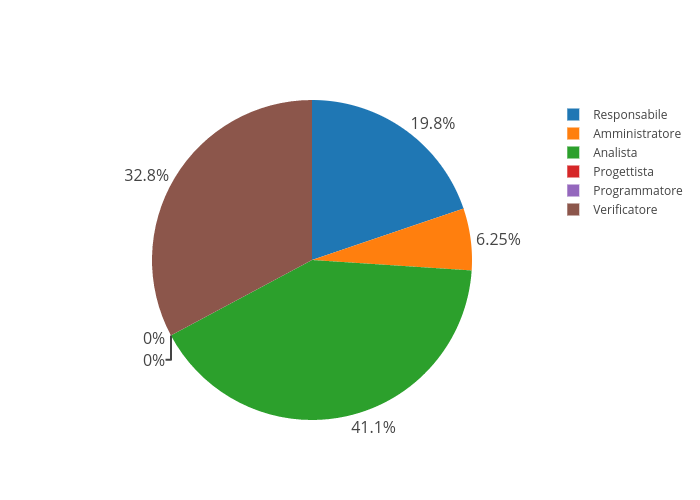
\includegraphics[scale=0.6]{img/AnalisiRequisiiti.png}
	\caption{Incidenza ore per ruolo, periodo di Analisi dei Requisiti}
\end{figure}

\subsection{Periodo di Analisi dei Requisiti Dettagliata}
La seconda porzione di Analisi dei Requisiti, da svolgersi dopo la Revisione dei Requisiti, è l'Analisi dei Requisiti Dettagliata. Come per il precedente, esso è da considerarsi parte dell'investimento intrapreso e quindi non è rendicontabile ai fini di calcolo del preventivo. Le ore totali sono XXX, suddivise come segue:

\begin{table}[H]
	\begin{center}
		\begin{tabular}{|c|c|c|}
			\hline
			\textbf{Ruolo}	& \textbf{Ore}	& \textbf{Ore remunerabili} \\
			\hline
			\Res	&	&  0\\
			\hline
			\Amm	&	&  0	\\
			\hline
			\Ana	&	&  0	\\
			\hline
			\Ver	&	&  0	\\
			\hline
		\end{tabular}
	\end{center}
	\caption{Ore per ruolo, periodo di Analisi dei Requisiti}
\end{table}

L'incidenza di tali ore determina in percentuale come mostrato di seguito:
\begin{figure}[H]
	\centering
	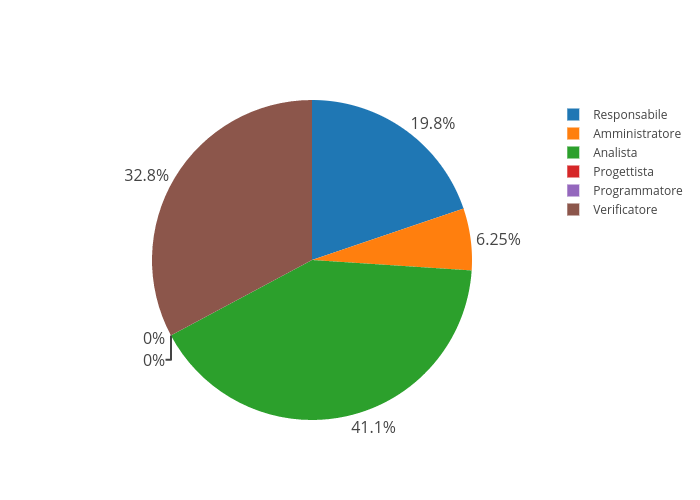
\includegraphics[scale=0.6]{img/AnalisiRequisiiti.png}
	\caption{Incidenza ore per ruolo, periodo di Analisi dei Requisiti}
\end{figure}

\subsection{Periodo di Progettazione Architetturale}
Lo sviluppo procede con la Progettazione Architetturale. Le ore totali sono 200, suddivise come segue:

\begin{table}[H]
	\begin{center}
		\begin{tabular}{|c|c|c|}
			\hline
			\textbf{Ruolo}	& \textbf{Ore}	& \textbf{Ore remunerabili} \\
			\hline
			\Res	&	5	&	5	\\
			\hline
			\Amm	&	5	&	5	\\
			\hline
			\Prog   &	138   &	138	\\
			\hline
			\Ver	&	52	&	52	\\
			\hline
		\end{tabular}
	\end{center}
	\caption{Ore per ruolo, periodo di Progettazione Architetturale}
\end{table}

L'incidenza di tali ore determina in percentuale come mostrato di seguito:
\begin{figure}[H]
	\centering
	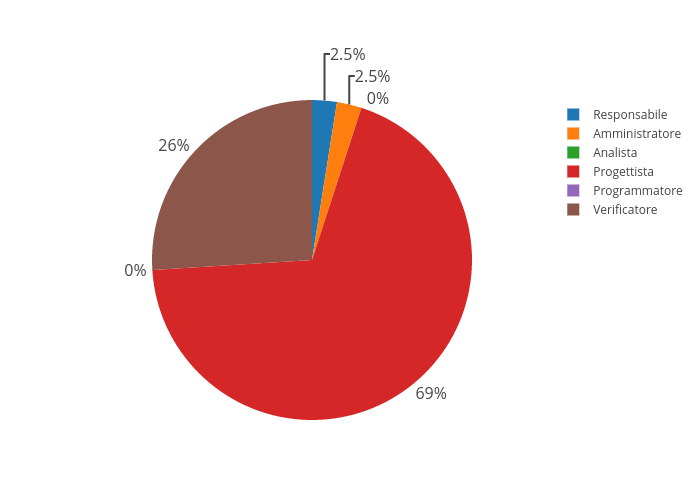
\includegraphics[scale=0.6]{img/ProgettazioneArchitetturale.png}
	\caption{Incidenza ore per ruolo, periodo di Progettazione Architetturale}
\end{figure}

\subsection{Periodo di Progettazione Architetturale Dettagliata}
Il terzo periodo è la Progettazione Architetturale Dettagliata. Le ore totali sono 118, suddivise come segue:

\begin{table}[H]
	\begin{center}
		\begin{tabular}{|c|c|c|}
			\hline
			\textbf{Ruolo}	& \textbf{Ore}	& \textbf{Ore remunerabili} \\
			\hline
			\Res	&	5	&	5 \\
			\hline
			\Amm	&	6	&	6	\\
			\hline
			\Prog   &	72   &	72	\\
			\hline
			\Ver	&	35	&	35	\\
			\hline
		\end{tabular}
	\end{center}
	\caption{Ore per ruolo, periodo di Progettazione Architetturale Dettagliata}
\end{table}

L'incidenza di tali ore determina in percentuale come mostrato di seguito:
\begin{figure}[H]
	\centering
	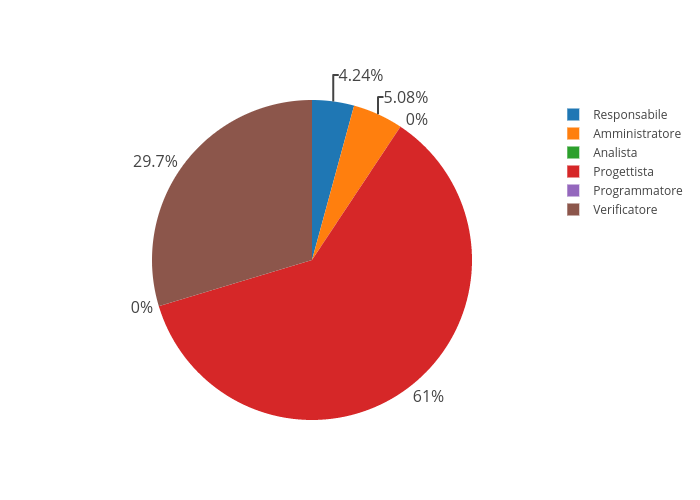
\includegraphics[scale=0.6]{img/ProgettazioneDettaglio.png}
	\caption{Incidenza ore per ruolo, periodo di Progettazione Architetturale Dettagliata}
\end{figure}

\subsection{Periodo di Codifica}
Il penultimo periodo è la Codifica. Le ore totali sono 213, suddivise come segue:

\begin{table}[H]
	\begin{center}
		\begin{tabular}{|c|c|c|}
			\hline
			\textbf{Ruolo}	& \textbf{Ore}	& \textbf{Ore remunerabili} \\
			\hline
			\Res	&	6	&	6	\\
			\hline
			\Amm	&	3	&	3	\\
			\hline
			\Progr   &	143   &	143	\\
			\hline
			\Ver	&	61	&	61	\\
			\hline
		\end{tabular}
	\end{center}
	\caption{Ore per ruolo, periodo di Codifica}
\end{table}

L'incidenza di tali ore determina in percentuale come mostrato di seguito:
\begin{figure}[H]
	\centering
	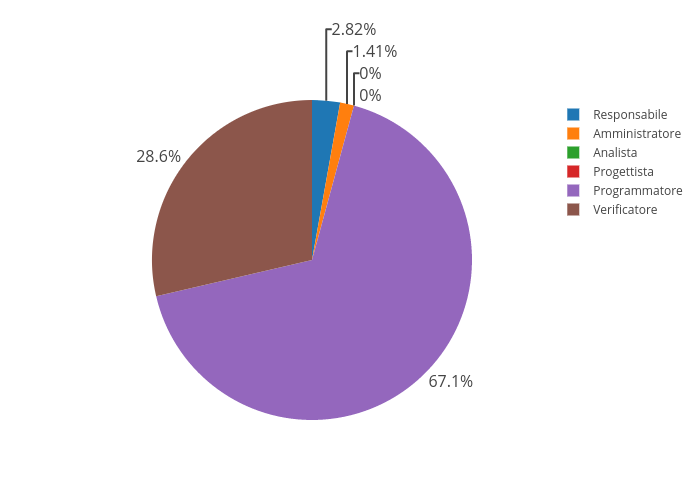
\includegraphics[scale=0.6]{img/Codifica.png}
	\caption{Incidenza ore per ruolo, periodo di Codifica}
\end{figure}

\subsection{Periodo di Verifica e Validazione}
L'ultimo periodo è la Verifica del prodotto sviluppato. Le ore totali sono 99, suddivise come segue:

\begin{table}[H]
	\begin{center}
		\begin{tabular}{|c|c|c|}
			\hline
			\textbf{Ruolo}	& \textbf{Ore}	& \textbf{Ore remunerabili} \\
			\hline
			\Res	&	6  &	6	\\
			\hline
			\Prog   &	15  &	15	\\
			\hline
			\Ver	&	78	&	78	\\
			\hline
		\end{tabular}
	\end{center}
	\caption{Ore per ruolo, periodo di Verifica e Validazione}
\end{table}

L'incidenza di tali ore determina in percentuale come mostrato di seguito:
\begin{figure}[H]
	\centering
	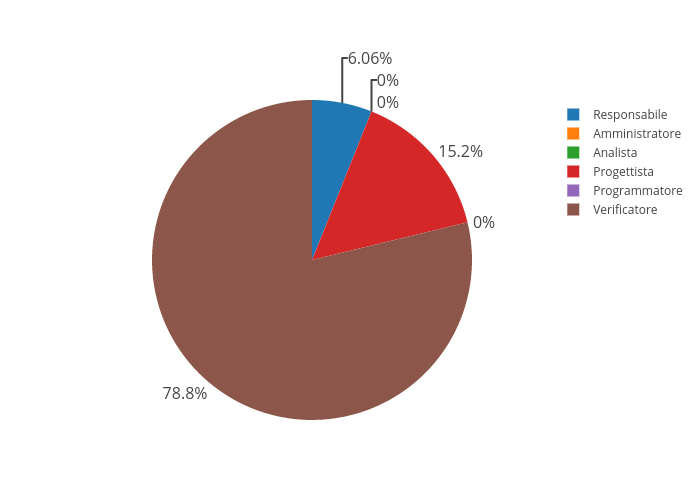
\includegraphics[scale=0.6]{img/Validazione.png}
	\caption{Suddivisione ore per ruolo, periodo di Verifica e Validazione}
\end{figure}

\subsection{Riepilogo}
Le ore totali del necessarie allo sviluppo sono 822 di cui, scorporando la fase di Analisi dei Requisiti, 630 remunerabili. Complessivamente le ore sono suddivise come segue:

\begin{table}[H]
	\begin{center}
		\begin{tabular}{|c|c|c|}
			\hline
			\textbf{Ruolo}	& \textbf{Ore complessive} & \textbf{Ore remunerabili} \\
			\hline
			\Res	&	57	&	19	\\
			\hline
			\Amm	&	29	&	17	\\
			\hline
			\Ana	&	79	&	0	\\
			\hline
			\Prog	&	225	&	225	\\
			\hline
			\Progr	&	143	&	143	\\
			\hline
			\Ver	&	289	&	226	\\
			\hline
		\end{tabular}
	\end{center}
	\caption{Ore per ruolo, Riepilogo}
\end{table}

L'incidenza di tali ore incide in percentuale come mostrato di seguito, prima complessive e poi remunerative:
\begin{figure}[H]
	\centering
	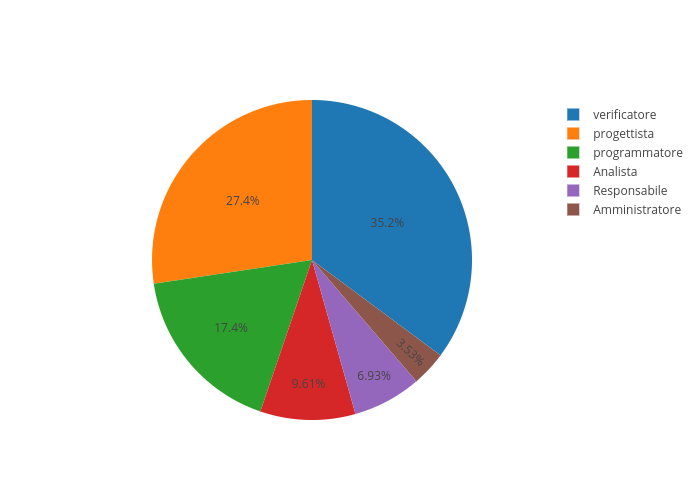
\includegraphics[scale=0.6]{img/OreTotali.png}
	\caption{Suddivisione ore per ruolo, riepilogo totale}
\end{figure}
\begin{figure}[H]
	\centering
	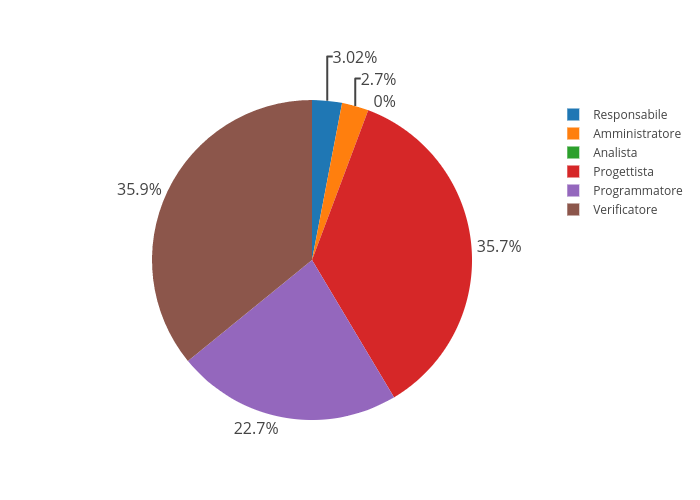
\includegraphics[scale=0.6]{img/OreRendicontabili.png}
	\caption{Suddivisione ore per ruolo, riepilogo ore remunerabili}
\end{figure}


\newpage

% template tabella!! Da cancellare solo quando finito
%\begin{table}[H]
%	\begin{center}
%		\begin{tabular}{|c|c|c|c|c|c|c|c|}
%			\hline
%			\textbf{nome} & \multicolumn{6}{c|}{\textbf{Ore per ruolo}} & \textbf{Ore totali} \\\cline{2-7}
%			& \textbf{Resp} & \textbf{Amm} & \textbf{An} & \textbf{Proj} & \textbf{Prog} & \textbf{Ver} & \\
%			\hline
%			\MC			&		&		&		&		&		&		&		\\
%			\hline
%			\AN			&		&		&		&	 	&		&		& 		\\
%			\hline
%			\DAN		&		&		&		&		&		&		&		\\
%			\hline
%			\AS			&		&	 	&	 	&		&	 	& 		&		\\
%			\hline
%			\NS 		&		&		&		&		&		& 		&		\\
%			\hline
%			\DS			& 		&		&		&		&		&		&		\\
%			\hline
%		\end{tabular}
%	\end{center}
%	\caption{Ore per componente, \AdR}
%\end{table}


\section{Registro Suddivisione Lavoro}
Nei seguenti paragrafi verrà spiegato come il gruppo intende dividere soddisfare alcune regole del progetto:
\begin{itemize}
	\item Tutti i componenti devono ricoprire almeno una volta tutti i ruoli; 
	\item Un componente del gruppo può ricoprire più ruoli contemporaneamente, purchè non entri in conflitto d'interesse, ad esempio non può Verificare il lavoro da lui svolto.
\end{itemize}

\subsection{Periodo di Analisi dei Requisiti}
Durante il periodo di \AdR, il lavoro dei membri sarà suddiviso come segue:

\begin{table}[H]
	\begin{center}
		\begin{tabular}{|c|c|c|c|c|c|c|c|}
			\hline
			\textbf{Nome} & \multicolumn{6}{c|}{\textbf{Ore per ruolo}} & \textbf{Ore totali} \\\cline{2-7}
			& \textbf{Resp} & \textbf{Amm} & \textbf{An} & \textbf{Proj} & \textbf{Prog} & \textbf{Ver} & \\
			\hline
			\MC			&		&		&	16	&		&		&	16	&	32	\\
			\hline
			\AN			&		&	4	&	6	&	 	&		&	22	& 	32	\\
			\hline
			\DAN		&		&	3	&	29	&		&		&		&	32	\\
			\hline
			\AS			&	20	&	 	&	12 	&		&	 	& 		&	32	\\
			\hline
			\NS 		&	18	&	3	&	11	&		&		& 		&	32	\\
			\hline
			\DS			& 		&	2	&	5	&		&		&	25	&	32	\\
			\hline
		\end{tabular}
	\end{center}
	\caption{Ore per componente, \AdR}
\end{table}

\begin{figure}[H]
	\centering
	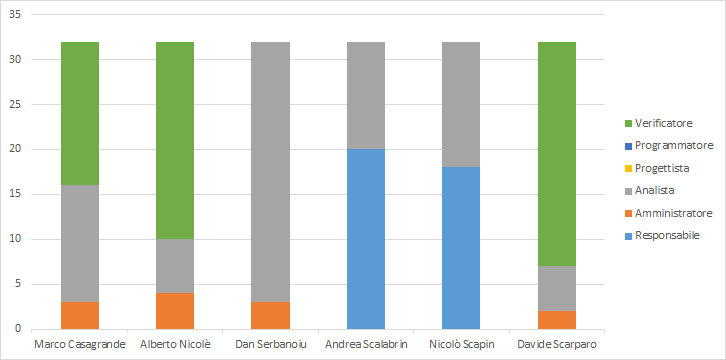
\includegraphics[scale=0.6]{img/6-1.png}
	\caption{Suddivisione ruoli per componente, Analisi dei Requisiti}
\end{figure}

\subsection{Periodo di Progettazione Architetturale}
Durante il periodo di progettazione architetturale, il lavoro dei membri sarà suddiviso come segue:

\begin{table}[H]
	\begin{center}
		\begin{tabular}{|c|c|c|c|c|c|c|c|}
			\hline
			\textbf{Nome} & \multicolumn{6}{c|}{\textbf{Ore per ruolo}} & \textbf{Ore totali} \\\cline{2-7}
			& \textbf{Resp} & \textbf{Amm} & \textbf{An} & \textbf{Proj} & \textbf{Prog} & \textbf{Ver} & \\
			\hline
			\MC			&		&	3	&		&	31	&		&		&   34	\\
			\hline
			\AN			&	3	&		&		&	31	&		&		& 	34	\\
			\hline
			\DAN		&		&	2	&		&	17	&		&	14	&	33	\\
			\hline
			\AS			&		&	 	&	 	&	14	&	 	& 	19	&	33	\\
			\hline
			\NS 		&		&		&		&	14	&		& 	19	&	33	\\
			\hline
			\DS			& 	2	&		&		&	31	&		&		&	33	\\
			\hline
		\end{tabular}
	\end{center}
	\caption{Ore per componente, Progettazione Architetturale}
\end{table}

\begin{figure}[H]
	\centering
	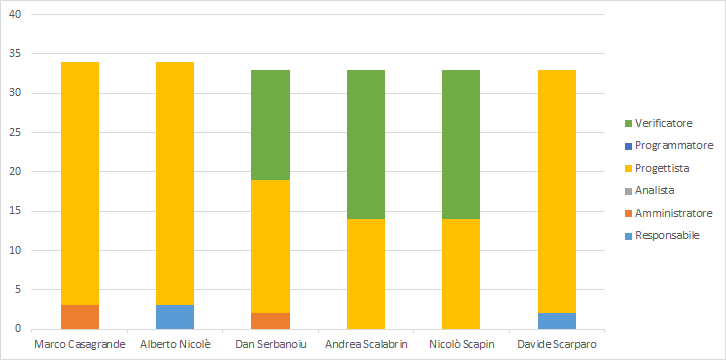
\includegraphics[scale=0.6]{img/6-2.png}
	\caption{Suddivisione ruoli per componente, Progettazione Architetturale}
\end{figure}

\subsection{Periodo di Progettazione Architetturale Dettagliata}
Durante il periodo di progettazione architetturale, il lavoro dei membri sarà suddiviso come segue:

\begin{table}[H]
	\begin{center}
		\begin{tabular}{|c|c|c|c|c|c|c|c|}
			\hline
			\textbf{Nome} & \multicolumn{6}{c|}{\textbf{Ore per ruolo}} & \textbf{Ore totali} \\\cline{2-7}
			& \textbf{Resp} & \textbf{Amm} & \textbf{An} & \textbf{Proj} & \textbf{Prog} & \textbf{Ver} & \\
			\hline
			\MC			&	2	&		&		&	6	&		&	11	&	19	\\
			\hline
			\AN			&		&		&		&	8	&   	&	11	& 	19	\\
			\hline
			\DAN		&	3	&		&		&	17	&		&		&	20	\\
			\hline
			\AS			&		&	3	&	 	&	17	&	 	& 		&	20	\\
			\hline
			\NS 		&		&	3	&		&	17	&		& 		&	20	\\
			\hline
			\DS			& 		&		&		&	7	&		&	13	&	20	\\
			\hline
		\end{tabular}
	\end{center}
	\caption{Ore per componente, Progettazione Architetturale Dettagliata}
\end{table}

\begin{figure}[H]
	\centering
	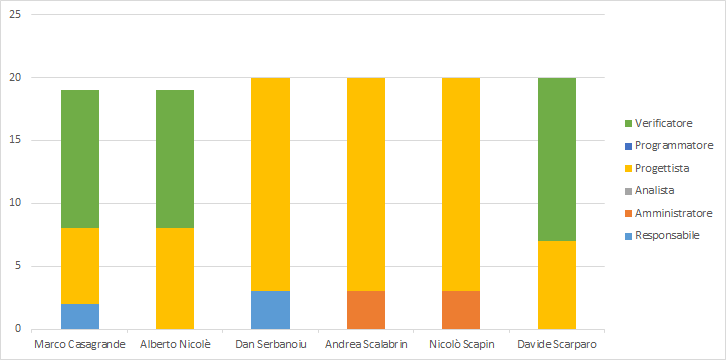
\includegraphics[scale=0.6]{img/6-3.png}
	\caption{Suddivisione ruoli per componente, Progettazione Architetturale Dettagliata}
\end{figure}

\subsection{Periodo di Codifica}
Durante il periodo di codifica, il lavoro dei membri sarà suddiviso come segue:

\begin{table}[H]
	\begin{center}
		\begin{tabular}{|c|c|c|c|c|c|c|c|}
			\hline
			\textbf{Nome} & \multicolumn{6}{c|}{\textbf{Ore per ruolo}} & \textbf{Ore totali} \\\cline{2-7}
			& \textbf{Resp} & \textbf{Amm} & \textbf{An} & \textbf{Proj} & \textbf{Prog} & \textbf{Ver} & \\
			\hline
			\MC			&		&		&		&		&	18	&	18	&	36	\\
			\hline
			\AN			&	3	&		&		&	 	&	32	&		& 	35	\\
			\hline
			\DAN		&		&		&		&		&	14	&	21	&	35	\\
			\hline
			\AS			&		&	 	&	 	&		&	14 	& 	22	&	36	\\
			\hline
			\NS 		&		&	3	&		&		&	32	& 		&	35	\\
			\hline
			\DS			& 	3	&		&		&		&	33	&		&	36	\\
			\hline
		\end{tabular}
	\end{center}
	\caption{Ore per componente, Codifica}
\end{table}

\begin{figure}[H]
	\centering
	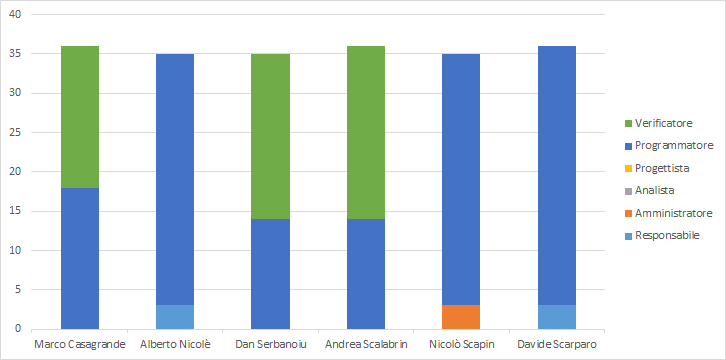
\includegraphics[scale=0.6]{img/6-4.png}
	\caption{Suddivisione ruoli per componente, Codifica}
\end{figure}

\subsection{Periodo di Verifica}
Durante il periodo di verifica, il lavoro dei membri sarà suddiviso come segue:

\begin{table}[H]
	\begin{center}
		\begin{tabular}{|c|c|c|c|c|c|c|c|}
			\hline
			\textbf{Nome} & \multicolumn{6}{c|}{\textbf{Ore per ruolo}} & \textbf{Ore totali} \\\cline{2-7}
			& \textbf{Resp} & \textbf{Amm} & \textbf{An} & \textbf{Proj} & \textbf{Prog} & \textbf{Ver} & \\
			\hline
			\MC			&		&	3	&		&	7	&		&	6	&	16	\\
			\hline
			\AN			&		&		&		&	 	&		&	17	& 	17	\\
			\hline
			\DAN		&	3	&		&		&		&		&	14	&	17	\\
			\hline
			\AS			&		&	 	&	 	&	4	&	 	& 	12	&	16	\\
			\hline
			\NS 		&		&		&		&	4	&		& 	13	&	17	\\
			\hline
			\DS			& 		&		&		&		&		&	16	&	16	\\
			\hline
		\end{tabular}
	\end{center}
	\caption{Ore per componente, Verifica}
\end{table}

\begin{figure}[H]
	\centering
	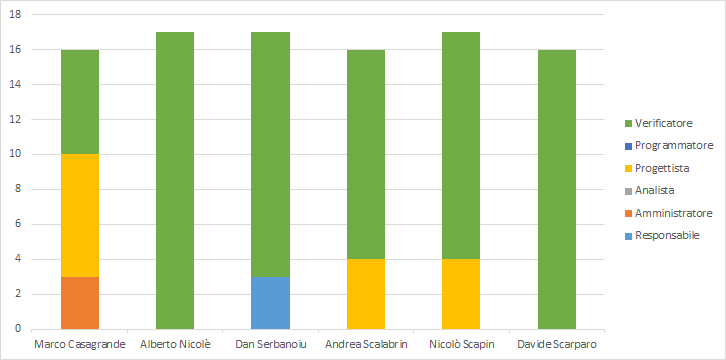
\includegraphics[scale=0.6]{img/6-5.png}
	\caption{Suddivisione ruoli per componente, Verifica}
\end{figure}

\subsection{Ore totali per componente}
Il consuntivo delle ore totali raggruppate per ciascun membro del gruppo, e suddiviso per il ruolo assunto durante tutte le fasi del progetto, risulta essere così suddiviso:

\begin{table}[H]
	\begin{center}
		\begin{tabular}{|c|c|c|c|c|c|c|c|}
			\hline
			\textbf{Nome} & \multicolumn{6}{c|}{\textbf{Ore per ruolo}} & \textbf{Ore totali} \\\cline{2-7}
			& \textbf{Resp} & \textbf{Amm} & \textbf{An} & \textbf{Proj} & \textbf{Prog} & \textbf{Ver} & \\
			\hline
			\MC			&	2	&	6	&	16	&	44	&	18	&	51	&	137	\\
			\hline
			\AN			&	6	&	4	&	6	&	39	&	32	&	50	& 	137	\\
			\hline
			\DAN		&	6	&	5	&	29	&	34	&	14	&	49	&	137	\\
			\hline
			\AS			&	20	&	3 	&	12 	&	35	&	14 	& 	53	&	137	\\
			\hline
			\NS 		&	18	&	9	&	11	&	35	&	32	& 	32	&	137	\\
			\hline
			\DS			& 	5	&	2	&	5	&	38	&	33	&	54	&	137	\\
			\hline
		\end{tabular}
	\end{center}
	\caption{Ore totali, per componente}
\end{table}

\subsection{Ore totali remunerabili}
La tabella sottostante, infine, raccoglie il conteggio complessivo delle ore remunerabili suddivise per ruolo e per ciascun componente.

\begin{table}[H]
	\begin{center}
		\begin{tabular}{|c|c|c|c|c|c|c|c|}
			\hline
			\textbf{Nome} & \multicolumn{6}{c|}{\textbf{Ore per ruolo}} & \textbf{Ore totali} \\\cline{2-7}
			& \textbf{Resp} & \textbf{Amm} & \textbf{An} & \textbf{Proj} & \textbf{Prog} & \textbf{Ver} & \\
			\hline
			\MC			&	2	&	6	&	0	&	44	&	18	&	35	&	105	\\
			\hline
			\AN			&	6	&	0	&	0	&	39	&	32	&	28	& 	105	\\
			\hline
			\DAN		&	6	&	2	&	0	&	34	&	14	&	49	&	105	\\
			\hline
			\AS			&	0	&	3 	&	0 	&	35	&	14 	& 	53	&	105	\\
			\hline
			\NS 		&	0	&	6	&	0	&	35	&	32	& 	32	&	105	\\
			\hline
			\DS			& 	5	&	0	&	0	&	38	&	33	&	29	&	105	\\
			\hline
		\end{tabular}
	\end{center}
	\caption{Ore totali remunerabili, per componente}
\end{table}



\end{document}